\documentclass[11pt,a4j,fleqn]{jarticle}
\usepackage{amsmath,amsthm,amssymb}
\usepackage[dvipdfmx]{graphicx}

\title{包絡線定理レポート}
\author{大野 嵩侃}
\date{2014年6月7日}


\begin{document}

\maketitle

\section{はじめに}
経済学における比較静学では, 長期と短期の関係をはじめ, 包絡線を用いて考える機会が多々あり, 包絡線定理はその重要な分析手法の1つである.

このレポートでは, まず包絡線の定義について具体例を交えて説明したのち, 包絡線定理について簡単な導入を行う.

また, 包絡線の概形をつかむため, 任意の曲線群についてパラメタを変化させたものをいくつか平面上にプロットした図を描いた. この図を描画するためにPythonを用いて書かれたコードに関しても説明する.

\section{包絡線定理}

\subsection{包絡線の求め方}
$x$をパラメタとする(微分可能な)関数$f(a,x)$について,$x$をある値$x_1$に固定すれば,$b=f(a,x_1)$を満たすような$a$と$b$の関係を表す曲線が1つ定まる.

同様に, $x$を$x_2$に固定すれば,$b=f(a,x_2)$を満たすような$a$と$b$の関係を表す曲線がやはり1つ定まる.

このように, $x$の値を変化させることで異なる曲線が定められるので,$b=f(a,x)$は$x$をパラメタとする$a-b$平面上の曲線群を表していると考えられる.

$x$を連続的に変化させると,この曲線の形も連続的に変化する.

ここで, ある曲線$b=g(a)$が$b=f(a,x)$で表されるすべての曲線と接していて, かつ接点の軌跡となっているとき,$g(x)$を$f(a,x)$の包絡線という.


この包絡線を求める方法について, 簡単な関数を用いて具体的に考えてみよう.
\begin{equation}
f(a, x) = x a - x^2\label{eq:1}
\end{equation}
とする. \eqref{eq:1}式の右辺を平方完成すると
\begin{equation}
f(a,  x) = -\left(x - \frac{a}{2}\right)^2 + \frac{a^2}{4} \label{eq:2}
\end{equation}
と変形できる. 式\eqref{eq:2}より, 
\begin{equation} 
\max_{x}f(a, x) = \frac{a^2}{4} \label{eq:3}
\end{equation}

よって, $x$にさまざまな値を代入して$a-b$グラフ上に描かれる複数の直線について, その包絡線$g(a)$は
\begin{equation} 
g(a) = \frac{a^2}{4} \label{eq:4}
\end{equation}
と表されると考えられる.

今回, $b=f(a, x)$は$x$を固定して考えると$a-b$平面上の直線を表すので, 求めた曲線$b=g(a)$上の任意の点における接線は, $b=f(a, x)$において$x$に何らかの値を代入して得られる$a-b$平面上の直線と一致するはずである.

実際にやってみよう.
\begin{equation} 
g'(a) = \frac{a}{2} \label{eq:5}
\end{equation}
であるから, 放物線$b=\frac{1}{4}a^2$上の点$(a_0,\frac{1}{4}{a_0}^2 )$における接線を$l(a_0)$とおくと\\
\begin{equation} 
l(a_0)=\frac{a_0}{2}(a-a_0)+\frac{{a_0}^2}{4}=\frac{a_0 \cdot a}{2} - \frac{{a_0}^2}{4} \label{eq:6}
\end{equation}
と表される. \eqref{eq:1}式と\eqref{eq:6}式を比較して, 
\begin{equation*} 
x = \frac{a_0}{2}
\end{equation*}
のとき, 確かに$f(a,  x)$は$a=a_0$における$b=g(a)$の接線を表している.

よって, $b=g(a)$は$b=f(a,x)$の包絡線であるといえる.

具体的に$x$の値をいくつかとって直線を重ねてみると, たしかに求めた$g(a)$に近い形が見えてくる.

たとえば$x$を$-2$から$2$まで$\frac{1}{3}$ずつ変化させて$13$本の直線を引いたものが図1, 
$x$を$-3$から$3$まで$\frac{1}{5}$ずつ変化させて$31$本の直線を引いたものが図2である.

より高い密度で広い範囲に接線を描いている分, 図2の方がより正確に$g(a)$を表わしているといえるが, 図1であっても$a$が0付近であれば十分$g(a)$に近いものが境界として描かれていることがわかるだろう.\\


\subsection{包絡線定理の説明とその直観的意味}
次に包絡線定理について述べる.

\eqref{eq:3}式の最大化問題の解は$a$に依存するので, その解を$x=x^* (a)$とおける.


$f(a,x^* (a))$で与えられる曲線は, 曲線群の包絡線$g(a)$に等しい.

よって, 次式が成り立つ.
\begin{equation}
\frac{d}{da}g(a)=\frac{d}{da}f(a,x^*(a))\label{eq:7}
\end{equation}

一方で, $f(a,x)$の$a$による偏導関数を定義すると, それに$(a,x)=(a,x^*(a))$を代入して得られる$b=f(a,x^* (a))$の接線の傾きは, 先に述べた包絡線の定義から$b=g(a)$の接線の傾きに等しい.

よって, 次式が成り立つ.
\begin{equation}
\frac{d}{da}g(a)=\frac{\partial f}{\partial a}(a, x^* (a)) \label{eq:8}
\end{equation}

包絡線定理とはこの\eqref{eq:8}式が, 変数$x,a$がともに多次元である場合も含めて常に成り立つというものである.

これが成立する理由についても述べておこう.

最適化問題の解においては, $x$の1要素をわずかに増減させても$f(a,x)$の値は変化しないことが知られている.

たとえば, 完全競争のもとで利潤を最大化しているとき, 生産コストと価格が(ほぼ)等しいためにある財$x_i$の生産をわずかに増減することは利潤の増減に(ほとんど)影響しない.

この事実を数式化した条件
\begin{equation*}
\frac{\partial f}{\partial x_i}(a,x^* (a))=0
\end{equation*}
を用いることで, \eqref{eq:7}式の右辺を\eqref{eq:8}式の右辺へと書き換えていくことができるのである.
\begin{figure}[p]
 \centering
 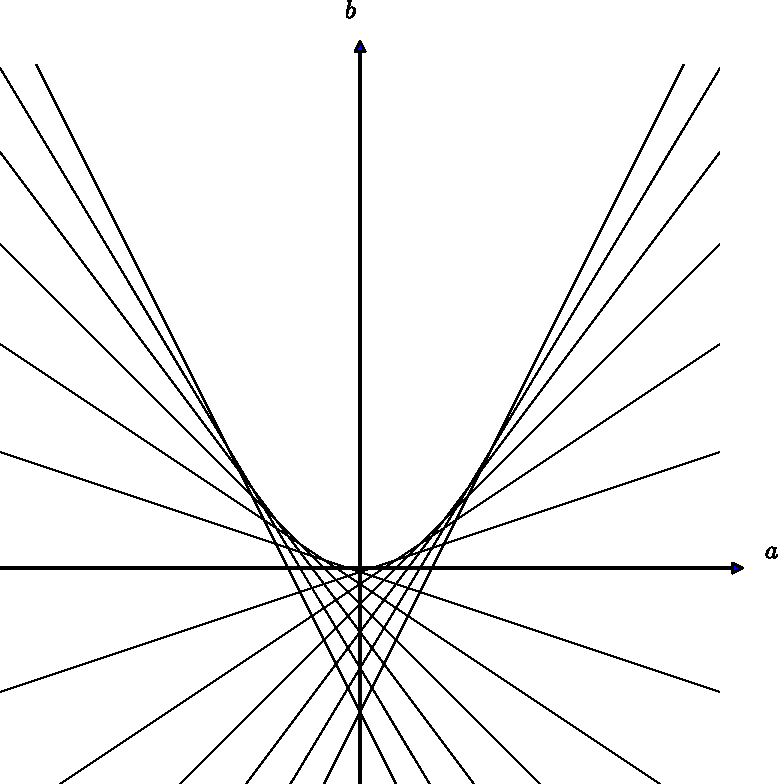
\includegraphics[scale=0.7]{envelope0.pdf}
 \caption{13本}
 \label{fig:1}
\end{figure}

\begin{figure}[p]
 \centering
 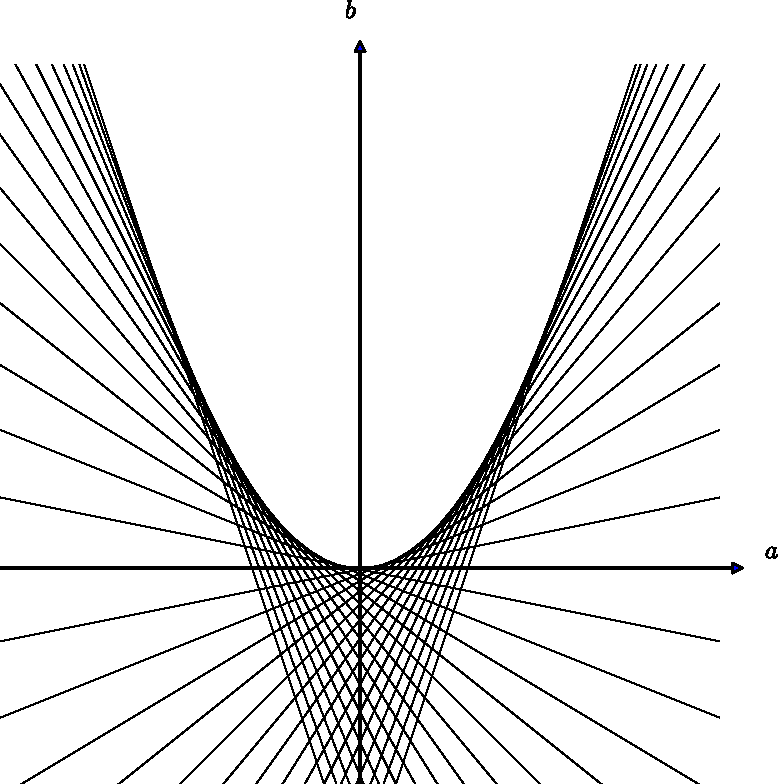
\includegraphics[scale=0.7]{envelope1.pdf}
 \caption{31本}
 \label{fig:2}
\end{figure}



\newpage
\section{Pythonプログラム}
\subsection{コード}
\begin{quote}
\begin{verbatim}
1  	from __future__ import division
2  	from numpy import linspace
3  	from numpy import array
4  	from mpl_toolkits.axes_grid.axislines import SubplotZero
5  	import matplotlib.pyplot as plt
6  	
7  	
8  	def f(x, a):
9  	    return a*x-x**2
10 	p = -3
11 	q = 3
12 	n = 12
13 	a_min = -10
14 	a_max = 10
15 	y_min = -6
16 	y_max = y_min+a_max-a_min
17 	plt.figtext(0.85, 0.35, '$a$')
18 	plt.figtext(0.5, 0.95, '$b$')
19 	fig = plt.figure(1)
20 	ax = SubplotZero(fig, 111)
21 	fig.add_subplot(ax)
22 	ax.axhline(linewidth=1.0, color="black")
23 	ax.axvline(linewidth=1.0, color="black")
24 	ax.set_xticks([])
25 	ax.set_yticks([])
26 	ax.set(aspect=1)
27 	for direction in ["xzero", "yzero"]:
28 	    ax.axis[direction].set_axisline_style("-|>")
29 	    ax.axis[direction].set_visible(True)
30 	plt.ylim(ymin=y_min)
31 	plt.ylim(ymax=y_max)
32 	a = linspace(a_min, a_max, (a_max-a_min) * 10)
33 	for i in range(n):
34 	    r = p+(q-p)*i/(n-1)
35 	    b = f(r, a)
36 	    ax.plot(a, b, 'k', linewidth=0.5, alpha=1)
37 	plt.show()
\end{verbatim}
\end{quote}

\subsection{コードの解説}
1~5行目では必要な機能を各モジュールからインポートした.

8~18行目にはこちらで入力する引数がまとめてある.詳細な情報は以下に記す.

8, 9行目では$x$をパラメタとする関数を定義している. $x$に具体的な値が代入されることで, $a-b$平面上の直線, あるいは曲線が表される.

10, 11行目で$x$に代入する値の最小値, 最大値をそれぞれp, qに入力する.

12行目では引く線の本数をnで定義した.

13, 14行目では, 出力する$a-b$グラフに表示させる$a$の最小値と最大値をそれぞれa\verb|_|min, a\verb|_|maxに入力する.

15, 16行目では, $a-b$グラフに表示させる$b$の最小値をy\verb|_|minに代入している. 
同様にy\verb|_|maxは$b$の最大値だが, 表示される$a$と$b$の幅が一致するよう自動で定まる.

17, 18行目では, 軸の名前となる文字(すなわち$a$と$b$)を位置を指定して埋め込んでいる.

19~29行目では軸を描いている.詳細は以下に記す.

19行目ではプロットすべきものの一覧を含んだデータ型の引数としてfigを定めている.この時点ではfigは空である.

20行目ではプロットすべきものそのものを表すデータ型の引数としてaxを定めている.

21行目でfigにaxを追加している.このとき, figの要素はaxのみである.

22~25行目ではaxに$a, b$軸を表すものを追加し, さらに軸に目盛りが入らないように目盛りを入れる位置を空のlistで指定している.

26行目ではグラフの縦横比を調整している
(初期設定だとプロットしたものがすべて表示されるよう自動で縮尺がいじられて縦長or横長になりうる)

27~29行目ではグラフの軸に矢印を追加している.

30, 31行目では"ylim"を用いてグラフの表示範囲を縦横で1:1にした. 
(そのままだと横方向に範囲が広いので, 正方形のグラフが出力されるように直している)

32~36行目では$x$に具体的な値を代入し, 得られる線についてグラフをプロットするという作業をn回繰り返しているため, 
最終的に$n$本の線がプロットされる.

37行目でプロットされたものを実際に表示して終了する.

\subsection{コードを書くにあたり工夫した点}
関数やそれによって描き出される包絡線の形が変化した時に対応しやすいよう, 
変化させうるところはモジュールをインポートしたすぐ後(9~18行目)にまとめてある.

また, 出力されるグラフが縮尺を$1:1$に保ちつつきれいな正方形を描くよう, "ylim"や"set(aspect=1)"などを用いた.

与えられる関数がaについて1次式である場合, 34行目では"array"を用いて2端点をとればよいが, 関数が1次式を表さない, 
すなわち曲線になる場合にも対応できるよう"linspace"を用いている. このため, 直線に特化したコードと比べると処理が遅くなる可能性はある.

\subsection{今後改善すべき点}
軸の名前の位置を現在は直接指定しているが, 軸の先に合わせる方法があるなら直すべきだろう.

また, 今回は$b=f(a,x)$が$x$固定時に直線を表す場合にも$a$の範囲を10倍した数の点をとっているが, これでは直線である場合に余分な作業をしている. 
場合分けを用いて, 直線時の作業では2端点をとるようにすることを考えたい.\\


\begin{thebibliography}{0}
\bibitem{}

\end{thebibliography}

\end{document}
